\section{kaneton event manager}

\subsection*{event interface}

\function{event\_reserve}{(i\_event \argument{id},
                           e\_event\_type \argument{type},
                           u\_event\_handler \argument{handler})}
	 {
	   This function installs an event handler.

	   \argument{type} can be :
	   \begin{itemize}
	     \item
	       \textbf{EVENT\_FUNCTION}: this means that the event will
	       call a function, which pointer is given in the union
	       \argument{handler}
	     \item
	       \textbf{EVENT\_MESSAGE}: this means that the event will
	       generate an IPC to the task given in the union
	       \argument{handler}.
	   \end{itemize}

	   The union \argument{handler} contains a pointer to a
	   function returning void and getting an event identifier in
	   argument and an optional error code (integer). The union
	   also contains a task identifier in the case of IPC action.
	 }

\function{event\_release}{(i\_event \argument{id})}
	 {
	   This function releases an event handler.
	 }

\subsection*{event manager example}

\begin{verbatim}
void          ia32_pf_handler(t_id         id,
                              t_uint32     error_code)
{
  t_uint32    addr;

  SCR2(addr);
  printf("#PF @ %p\n", addr);

  while (1)
    ;
}

...

event_reserve(14, EVENT_FUNCTION, EVENT_HANDLER(ia32_pf_handler));
\end{verbatim}

\newpage

\section{kaneton thread manager}

\subsection*{thread interface}

\function{thread\_reserve}{(i\_task \argument{task},
                            t\_prior \argument{prior},
                            i\_thread* \argument{id})}
	 {
	   This function reserves a thread for the task \argument{task}
	   given the default thread priority \argument{prior}.

	   Note that once reserved, the thread is marked as stopped.

	   The priority must be in the interval \emph{THREAD\_LPRIOR},
	   \emph{THREAD\_HPRIOR}.
	 }

\function{thread\_release}{(i\_thread \argument{id})}
	 {
	   This function releases the thread object \argument{id}.
	 }

\function{thread\_priority}{(i\_thread \argument{id},
                             t\_prior \argument{prior})}
	 {
	   This function updates the current thread priority
	   to \argument{prior}.

	   The priority must be in the interval \emph{THREAD\_LPRIOR},
	   \emph{THREAD\_HPRIOR}.
	 }

\function{thread\_state}{(i\_thread \argument{id},
                          t\_state \argument{sched})}
	 {
	   This function stops or starts a thread.

	   Values for \argument{sched} are:

	   \begin{itemize}
	     \item
	       \emph{SCHED\_STATE\_RUN}: run the thread.
	     \item
	       \emph{SCHED\_STATE\_STOP}: stop the thread.
	   \end{itemize}
	 }

\function{thread\_get}{(i\_thread \argument{id},
                        o\_thread** \argument{o})}
	 {
	   This function returns in \argument{o} the thread object
	   corresponding to \argument{id}.
	 }

\function{thread\_stack}{(i\_thread \argument{id},
                          t\_stack \argument{stack})}
	 {
	   This function allocates a stack for the thread \argument{id}.

	   The \argument{stack} argument is a struct containing the
	   size of the stack and a field called \emph{base}. If the
	   base is set to a value different of 0, then no space will
	   be allocated and the base of the stack will be set to the
	   address \argument{base}.
	 }

\function{thread\_load}{(i\_thread \argument{id},
                         t\_thread\_context \argument{context})}
	 {
	   This function loads a new execution context in the thread
	   object \argument{id}.

	   A thread execution context \textit{t\_thread\_context}
	   only contains the \textit{program counter} and the
	   \textit{stack pointer}.
	 }

\newpage

\section{kaneton sched manager}

\subsection*{sched interface}

\function{sched\_yield}{(i\_cpu \argument{cpuid})}
	 {
	   This function permits the current thread to relinquish
	   the processor voluntarily.

	   Do not care about the argument \argument{cpuid}.
	 }

\function{sched\_add}{(i\_thread \argument{thread})}
	 {
	   This function adds a runnable thread to the scheduler. Even
	   if the added thread has the highest priority, do not yield
	   the current thread.
	 }

\function{sched\_remove}{(i\_thread \argument{thread})}
	 {
	   This function removes a thread from the
	   scheduler. \textbf{Be careful:} the thread to remove can be
	   the currently executing thread.
	 }

\function{sched\_update}{(i\_thread \argument{thread})}
	 {
	   This function asks the scheduler to update the thread
	   \argument{thread} in its internal data structures since
	   for example the thread's priority just changed.
	 }

\function{sched\_current}{(i\_thread* \argument{thread})}
	 {
	   This function returns in \argument{thread} the identifier
	   of the thread currently executed.
	 }

\section{kaneton set manager}

\subsection*{set interface}

\function{set\_size}{(i\_set \argument{id},
                      t\_setsz \argument{size})}
	 {
	   This function returns in \argument{size} the number of elements
	   of the set.
	 }

\function{set\_add}{(i\_set \argument{id},
                     void* \argument{data})}
	 {
	   This function adds a data object in the set \argument{id}.
	 }

\function{set\_remove}{(i\_set \argument{id},
                        t\_id \argument{i})}
	 {
	   This function removes an object identified by \argument{i}
	   from the set \argument{id}.
	 }

\function{set\_object}{(i\_set \argument{id},
                        t\_iterator \argument{iterator},
                        void** \argument{data})}
	 {
	   This function returns the data object corresponding to
	   the iterator.
	 }

\function{set\_get}{(i\_set \argument{setid},
                     t\_id \argument{id},
                     void** \argument{o})}
         {
	   This function retrieve an element in the set given its
	   identifier \argument{id}.
	 }

\function{set\_push}{(i\_set \argument{id},
                      void* \argument{data})}
	 {
	   This function adds an object to a FIFO or LIFO structure.
	 }

\function{set\_pop}{(i\_set \argument{id})}
	 {
	   This function removes the next object of a FIFO or LIFO structure.
	 }

\function{set\_pick}{(i\_set \argument{id},
                      void** \argument{data})}
	 {
	   This function returns the next object of a FIFO or LIFO structure
	   without deleting it.
	 }

\function{set\_reserve}{(\argument{type},
                         t\_opts \argument{opts},
                         t\_size \argument{datasz},
                         i\_set* \argument{id})}
	 {
	   This function reserves a set object of type \argument{type}
	   with options \argument{opts} which will contain object of
	   \argument{datasz} size.

	   The reserved set object's identifier is returned in
	   \argument{id}.

	   Values for \argument{type} are:

	   \begin{itemize}
	     \item
	       \emph{ll}: doubly linked-list
	     \item
	       \emph{array}: array
	     \item
	       \emph{pipe}: FIFO
	     \item
	       \emph{stack}: LIFO
	   \end{itemize}
	 }

\function{set\_release}{(i\_set \argument{id})}
	 {
	   This function releases the set \argument{id}.
	 }

\subsection*{set\_foreach example}

\begin{verbatim}
t_state         state;
o_segment       *seg;
t_iterator      i;

set_foreach(SET_OPT_FORWARD, segments, &i, state)
  {
    if (set_object(segments, i, (void**)&seg) != ERROR_NONE)
      AS_LEAVE(as, ERROR_UNKNOWN);

    // use seg variable here
  }
\end{verbatim}

\newpage

\section{Feuille de r�ponse de l'excercice 3}

Nom :\hspace{5cm}Prenom :\\

\subsection{Round Robin avec priorit� et vieillisement}

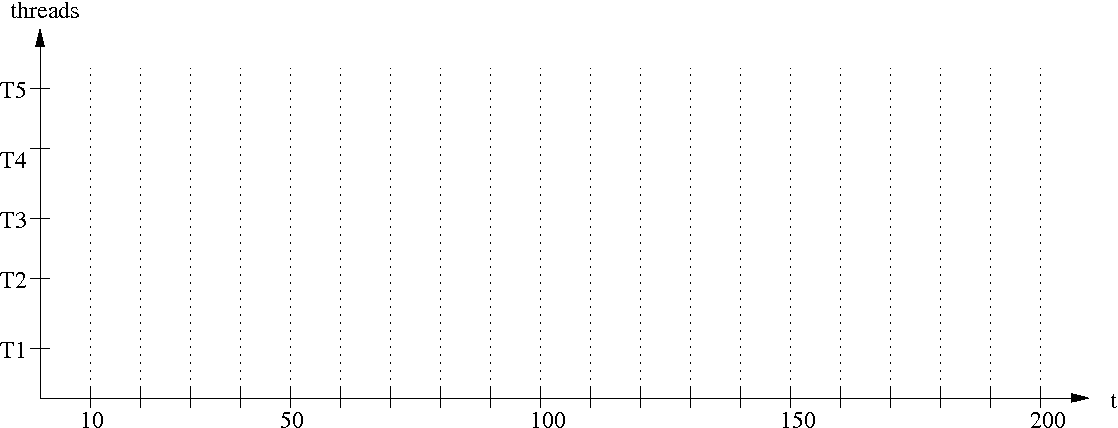
\includegraphics[width=\linewidth]{figures/grid-sched}

\subsection{Multilevel Feedback Queue}

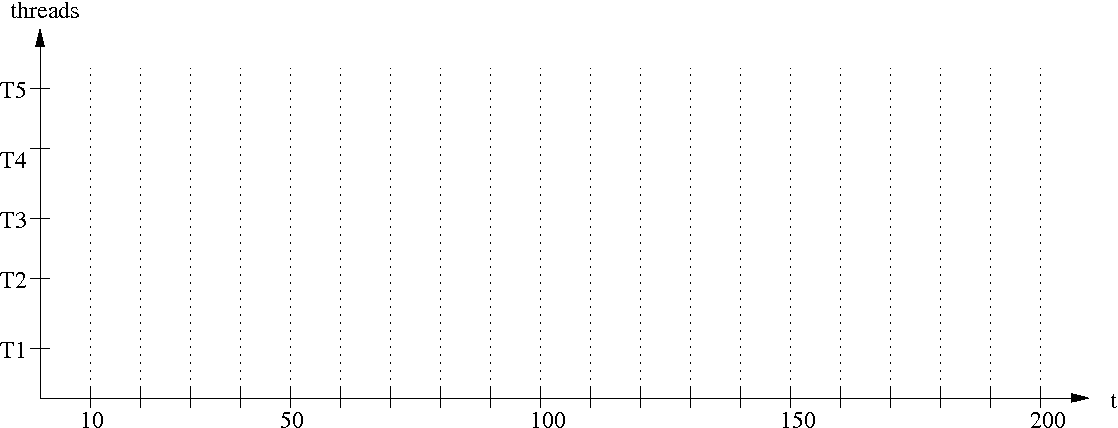
\includegraphics[width=\linewidth]{figures/grid-sched}

\newpage
\begin{correction}

\section{Feuille de r�ponse de l'excercice 3}

Nom :\hspace{5cm}Prenom :\\

\subsection{Round Robin avec priorit� et vieillisement}

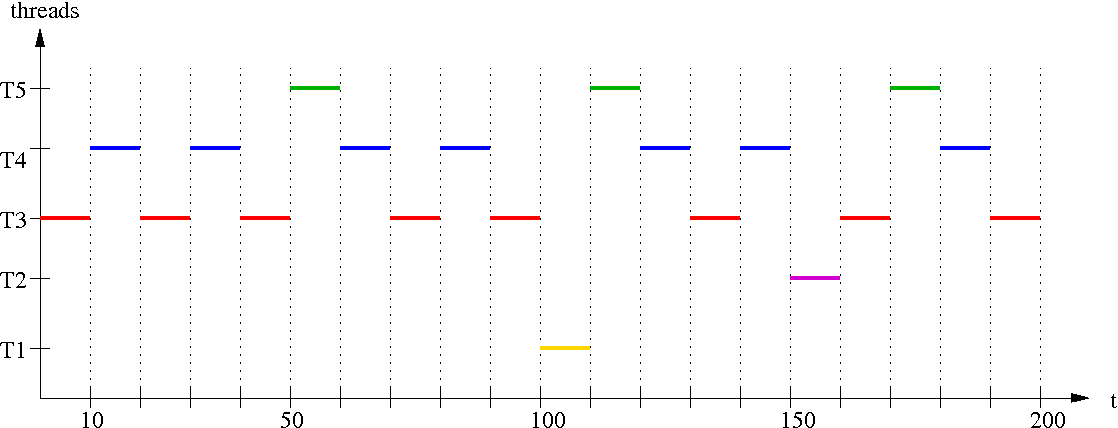
\includegraphics[width=\linewidth]{figures/grid-sched-rr}

\subsection{Multilevel Feedback Queue}

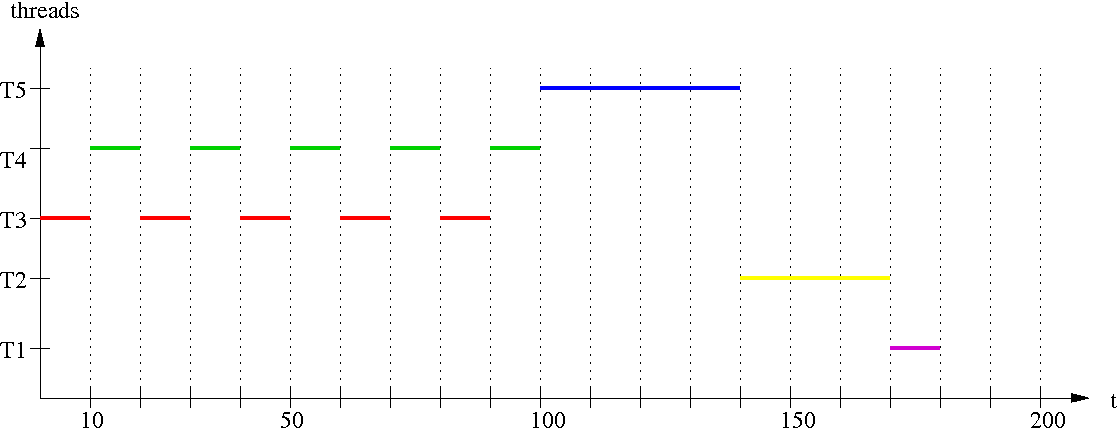
\includegraphics[width=\linewidth]{figures/grid-sched-mfq}
\end{correction}
\end{document}
